\chapter{总体架构设计}
\section{系统设计目标}
\subsection{高保真性}
本系统把高保真性当作核心目标之一,要求生成交通场景能最大程度忠实反映自然语言描述,为实现这一目标,系统不光要保证场景视觉效果和语义的一致性,还得考虑各种复杂环境要素和交通行为的准确性,就像生成场景里各类交通工具行为需和现实世界交通流动保持一致,交通规则和行为模式也得严格遵循,所以系统要对输入描述进行精确解析,运用先进自然语言处理技术(像大语言模型)来理解场景各种细节并转换为对应三维仿真环境,这些细节不只是物理上的位置和对象,还涵盖交通元素间的动态互动以及环境条件如天气时间光照等因素的考量。

\subsection{自动化}
本系统设计的另一个关键目标就是实现自动化,通过达成从自然语言输入到场景生成与仿真运行的自动化流程,系统能够减少人工干预情况,进而提高运行效率并降低人为错误的发生概率,系统要能够凭借少量的用户输入(比如一段简短的自然语言描述)来完成从场景构建直至仿真运行的全过程,自动生成所有必需的配置文件,调度仿真平台开展执行工作,并收集仿真结果用于后续分析处理,自动化并不局限于场景生成这一方面,还涵盖场景的评估以及结果展示等内容,能够在场景生成之后直接对其进行可视化与量化评估,并且输出最终的评估报告,这种全自动的流程会极大地提升仿真研究的工作效率,从而支持大规模的实验以及多样化的场景生成需求。

\subsection{可扩展性}
可扩展性在系统设计里是很重要的原则,要保证系统能随需求变化做功能和技术扩展,系统设计应该采用模块化的结构,像自然语言处理、场景生成等每个功能模块都能独立发展和优化,还可与其他模块实现无缝衔接,可扩展性体现在下面这几个方面
\begin{itemize}
	\item 自然语言处理模型要进行升级,伴随自然语言处理技术不断发展,新的语言模型与算法可能会持续出现,系统应具备灵活集成新语言模型的能力,以此提升场景生成的准确性和多样性。
	\item 仿真平台的集成方面目前当前平台采用CARLA作为仿真引擎不过未来可能会考虑集成其他仿真平台或者与不同的驾驶仿真系统进行对接以此来支持更多元的实验需求以及不同平台之间的比较。
	\item 系统评估模块要支持定制化与多维度评估指标,体现评估指标多样性,未来可依据不同场景类型、研究需求或者应用场景添加新评估标准,同时改进现有的评估方法。
\end{itemize}

\subsection{核心功能实现}
本系统的核心功能涵盖三个关键方面:
\begin{itemize}
	\item 从自然语言描述自动生成三维交通场景这个功能是系统基础,它的目的是通过理解输入的自然语言来自动生成可在仿真环境运行的交通场景,系统会利用自然语言处理模型以及检索增强技术,结合已有的场景模板和元素库实现语义精确的场景建模。
	\item 对生成的场景开展仿真和可视化操作,这个功能主要是保证生成的三维场景能够在仿真平台里正确呈现且顺利运行,系统借助调用仿真平台的API,自动把生成的场景描述转换为可执行的仿真环境,进而开展实时仿真与动态可视化工作,此过程还涵盖对场景中交通元素的行为进行模拟,比如交通流情况、车辆行驶轨迹以及交互状况等。
	\item 对生成结果开展量化评估工作,评估是本系统不可缺少的重要组成部分,它能提供对生成场景质量的定量分析内容。系统会依据语义保真度、场景多样性和驾驶性能等具体指标,开展评估工作并生成对应的报告文档。借助量化评估方式,系统可为场景生成给予反馈信息以便后续优化处理,同时为自动驾驶算法的性能测试提供参考依据。
\end{itemize}

\subsection{系统目标的长期愿景}
随着技术不断进步系统要逐步朝着更高保真度、更强可扩展性、更高效自动化方向发展,在未来的版本当中系统可以集成更多感知模型、智能决策系统等相关技术,以此进一步提升场景的复杂性以及真实性,同时系统的评估模块也能够通过引入更多智能分析工具,来提供像行为预测、决策模型评估等更细粒度的结果评估,此外伴随自然语言处理技术的进步系统能够处理更为复杂的语言输入和场景需求,从而满足更广泛的仿真测试场景需求并支撑更丰富的自动驾驶研究与开发。
\section{系统总体架构}
系统的整体架构就像图3 - 1\ref{fig:system_architecture}所展示的那样,主要是分成了三个核心的模块,分别是自然语言理解与场景生成模块、场景合成与仿真模块以及场景评估与展示模块,数据的流动过程如下
\begin{enumerate}
	\item 用户输入自然语言指令;
	\item 系统通过检索增强与大语言模型解析自然语言,生成对应的Scenic场景描述脚本;
	\item Scenic脚本由Scenic解析器处理,并通过CARLA仿真平台进行三维场景构建与动态仿真;
	\item 仿真完成后系统采集结果数据,包括场景截图与驾驶轨迹;
	\item 对生成场景进行量化评估,输出语义保真度、多样性与驾驶性能相关指标。
\end{enumerate}
\begin{figure}[H]
	\centering
	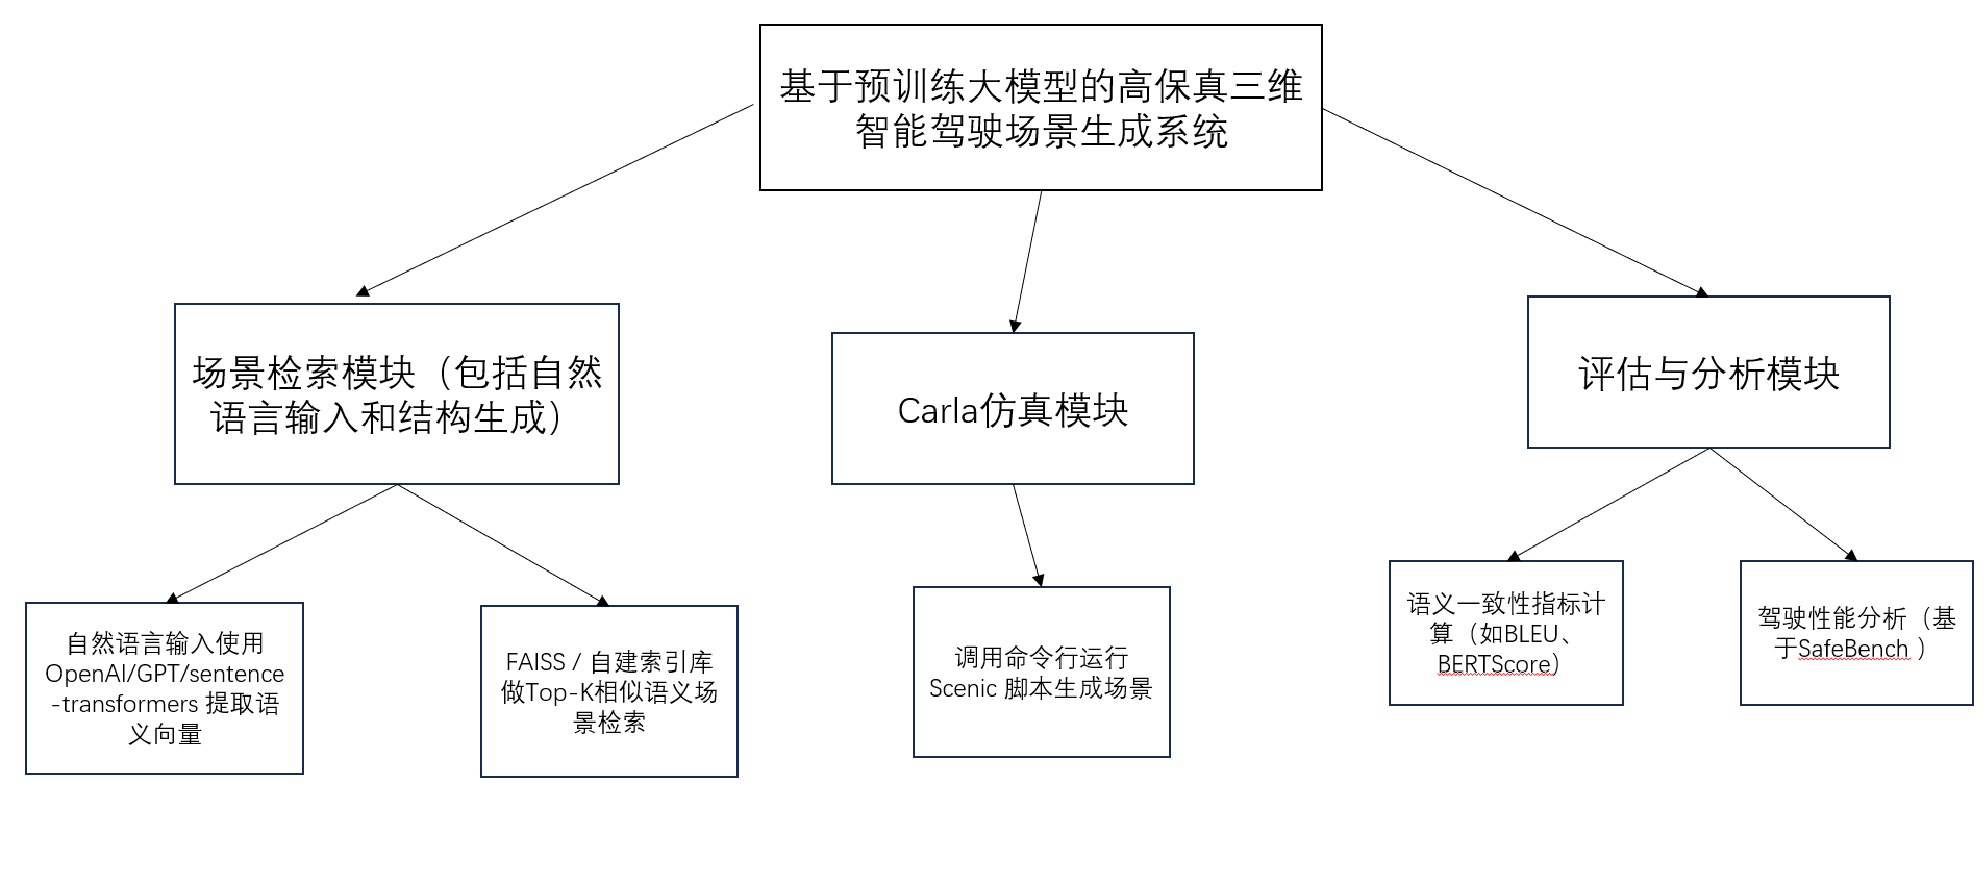
\includegraphics[width=0.9\textwidth]{../images/系统架构图.pdf} 
	\caption{系统架构图}
	\label{fig:system_architecture} % 添加合适的label
\end{figure}

\section{主要模块功能设计}
\subsection{自然语言理解与场景生成模块}
本模块负责接收自然语言输入并生成对应的Scenic场景描述。具体流程如下:
\begin{itemize}
	\item \textbf{输入}:自然语言形式的场景描述,例如“一个红色轿车在城市路口等待绿灯”。
	\item \textbf{检索增强}:使用 \texttt{sentence-transformers} 中的 \texttt{sentence-t5-large} 模型对输入进行向量化表示,并在本地检索数据库\\(如 \texttt{retrieve/scenario\_descriptions.txt})中查找相似描述作为参考样本。
	\item \textbf{大语言模型解析}:采用预训练的大语言模型(如 GPT-4o),结合检索到的参考样本,生成符合输入语义的 Scenic 脚本。
	\item \textbf{场景拼接机制}:根据场景复杂度,支持对多个子元素(如车辆、行人、环境条件)进行组织与拼接。
\end{itemize}


\subsection{场景合成与仿真模块}

本模块负责将自然语言生成的Scenic脚本转化为三维可视化仿真场景,并在CARLA仿真平台上实现动态运行。整个过程包括脚本解析、场景构建、仿真控制、交互支持与数据输出等多个环节,具体如下:

\begin{itemize}
	\item \textbf{Scenic解析}:本系统会先借助Scenic内置的语法与语义分析器来对输入脚本开展解析工作,Scenic作为一种领域专用语言可让用户用简洁且结构化的方式去描述场景元素像车辆、行人、障碍物等的初始状态和约束条件,解析过程能够生成涵盖对象属性如位置、速度、朝向以及交互规则如跟车距离、避让行为还有环境条件如天气、时间的完整场景配置
	
	\item \textbf{仿真构建}:完成脚本解析之后系统自动把Scenic生成中间配置映射到CARLA仿真平台里,具体涵盖载入指定地图、部署交通参与者、设定摄像头和LiDAR等传感器参数、配置天气光照路况等环境因素等内容,系统能够依据配置实现对城市道路高速公路十字路口等多种类型场景精准建模
	\item \textbf{接口调用关系}Scenic借助和CARLA集成的Python API来调用底层仿真接口,系统会自动完成Actor的创建以及状态初始化和行为脚本绑定等任务,这极大程度简化了从脚本到仿真的转换流程,研究人员不用手动编程就能通过文本控制仿真流程,显著提升了效率和复用性。
	
	\item \textbf{动态交互支持}:系统能够支持高度动态化的场景仿真工作,还可以模拟交通参与者之间的交互行为,像车辆变道、避障、红绿灯响应以及行人横穿马路等情况,Scenic语言提供了条件触发与时间控制相关机制,允许用户描述复杂的行为序列内容,以此实现具有时序性、可演化的场景变化状况,从而增强了仿真的真实感与复杂程度。
	
	\item \textbf{多样化仿真配置}:这个模块能够支持进行灵活的仿真参数配置,其中涵盖地图选择像Town01、Town05这类,还有天气设置包含晴天、雨天、雾天等情况,以及交通流量控制和车辆控制模式如自动驾驶、手动控制等内容,这样可以满足不同的测试需求,并且该模块还支持使用不同版本的CARLA和Scenic进行组合,具备较好的兼容性与可拓展性。
	
	\item \textbf{数据采集与输出}:在仿真执行的过程当中,系统能够实时采集关键数据,这些数据涵盖传感器输出(像RGB图像、深度图、点云等)、车辆状态(包含位置、速度、加速度)、交互事件(例如碰撞、刹车、偏航)等内容,采集到的数据可用于后续模型训练、行为评估或者性能对比等任务,以此支撑多种不同的研究方向。
	
\end{itemize}


\subsection{场景评估与展示模块}

场景评估与展示模块的目的是对生成的三维仿真场景做可视化呈现和定量分析,此模块方便研究人员直观了解场景生成具体效果,也为后续性能比较、模型调优以及系统验证提供评估依据,该模块包含下面几个关键功能:

\begin{itemize}
	\item \textbf{可视化展示}:在仿真进行的过程当中系统能够自动截取关键帧的截图,或者录制完整的仿真过程视频并保存成图像或视频文件,这些可供研究人员用来做人工审阅、可视化报告展示以及用户研究评估,截图一般会选择交通事件发生点像刹车、避障、碰撞等情况,或者特定的时序节点,以此确保所展示信息具备代表性与丰富性,视频部分可以借助CARLA原生录制功能或者集成第三方渲染引擎来实现,并且支持多角度、多摄像机的可视观察,从而进一步增强场景调试与验证方面的可操作性。
	
	\item \textbf{量化评估}:本系统是在自动化生成以及仿真的基础之上,进一步引入多维度的量化评估指标,以此对场景生成的有效性、合理性和多样性进行定量测量,具体涵盖的内容有:
	
	\begin{itemize}
		\item \textbf{语义保真度(Semantic Fidelity)}:这个指标的作用是衡量输入的自然语言描述和最终生成的仿真场景之间语义一致性,可采用人工标注评分和自动化匹配算法相结合的方式来开展,比如通过设定关键语义要素像地点、交通行为、天气条件等的匹配程度,对场景是否准确还原用户意图进行评分,自动方法能够结合自然语言处理与图结构匹配技术实现初步评估进而提升效率。
		

		\item \textbf{多样性指标(Scene Diversity)}:这项指标能反映系统生成场景在多次输入不同自然语言之后的差异性以及覆盖范围,主要涵盖空间多样性像不同地图位置与道路类型等方面、元素多样性比如参与车辆行人非机动车种类情况、行为多样性包含速度控制路线选择交通交互等内容,统计方法有使用Shannon熵、Jaccard相似度或者聚类分布指标等,以此全面反映生成系统的泛化能力和表现范围。
		
		\item \textbf{驾驶性能指标(Driving Performance)}:为了评估生成场景对自动驾驶系统测试价值,本模块支持在生成场景里运行预设自动驾驶控制系统,像基于CARLA的自动驾驶Agent并记录其表现,关键评估维度包含碰撞率也就是单位场景中发生碰撞的比例、任务成功率即是否成功完成任务或驶出场景、路径偏离率指与理想路径的偏差程度等,这些数据能够用于评估生成场景的挑战性与安全测试覆盖度,是场景质量评估的重要依据。
	\end{itemize}
	
	\item \textbf{评估结果展示与导出}:系统能够支持把评估结果用图表和表格等形式来做可视化展示,这样方便研究人员开展对比分析以及生成结果报告,所有截图、评估指标还有分析数据都可以导出成标准格式文件,例如CSV、JSON、PNG等,可用于论文撰写、模型调试或者进一步的数据挖掘。
	
\end{itemize}